\documentclass[12pt, a4paper,oneside]{report}
\usepackage{titlesec}
\usepackage[utf8]{inputenc}
\usepackage{german}
\usepackage[T1]{fontenc}
\usepackage{textcomp}
\usepackage{framed}
\usepackage{pbox}
\usepackage{caption}
\usepackage[nottoc,numbib]{tocbibind}
\usepackage[pdftex]{graphicx}
\usepackage[toc]{glossaries}
\usepackage{amssymb, amsmath}
\usepackage[colorlinks,
pdfstartview = FitH,
linkcolor = black,
plainpages = false,
hypertexnames = false,
citecolor = black]{hyperref}
\usepackage{setspace}
\onehalfspacing
\usepackage[left=3.5cm,right=3.5cm,top=2cm,bottom=2cm]{geometry}
\graphicspath{{./pics/}}
\usepackage[printonlyused]{acronym}
\usepackage{todonotes}
\usepackage{subcaption}
\usepackage{float}
\usepackage{pifont}
\newcommand{\cmark}{\ding{51}}%
\newcommand{\xmark}{\ding{55}}%
\usepackage{multirow}
\usepackage{pdflscape}
\usepackage{eurosym}
\usepackage{tocbibind}
\usepackage[english]{babel}
\usepackage[utf8]{inputenc}
\usepackage{multirow}
\usepackage{subcaption}

\begin{document}

\begin{titlepage}
	Universität Passau\newline
	Fakultät für Informatik und Mathematik
	\vspace{2.5cm}
    \begin{center}
    \LARGE\textbf{{Classification  Of Visualization  In Scientific Literature}}\\
   
    \normalsize

    \vspace{2.5cm}
    \end{center}

 \normalsize{
 	Masterarbeit zur Erlangung des akademischen Grades\newline
 	Master of Science (M.Sc.)\newline
 	\ \\
 	Lehrstuhl für Intelligent Systems und Lehrstuhl für Data Science \newline
 	der Fakultät für Informatik und Mathematik\newline
 	der Universität Passau\newline
 	
 
    \begin{tabular}{ll}
    	Name: & Arnold Azeem \\
    	Matrikelnummer: & 79176 \\
    	Fachbereich: & Informatik\\
    	Studiengang: & Master Informatik\\
	Erstprüfer: & Prof. Dr. Christin Siefert \\
	Zweitprüfer: & Prof. Dr. Michael Granitzer\\
	Date: &     \today
    \end{tabular}\\
    }



\newpage
\begin{abstract}
Distinct visualisation techniques are used in scientific research publications to summarise large amount of data and also represent a variety of data. These visualisations help to communicate complex information and support the arguments being presented in the publication in a way that is easy to understand and follow.
These figures tend to reveal trends, patterns or relations that might have otherwise been difficult to grasp using only text. 
It is therefore relevant that we extract the data from these visualisations since the extracted data can be used for validating the publication or presenting the data in another form for a different audience. In this context, classifying these visualisations is the initial step since, there is a variety of visualisations and each one is processed in a specific way. It is only after classification that extraction of raw data from these visualisations can be acquired for other tasks. This thesis presents an approach whereby real world data is used to create four types of plots (scatter plots, bar charts, line charts, and box-plots) and random plots also of the same kind from the Internet are added together and used to train and evaluate a CovNet model to be able to classify these plots. 
\end{abstract}

\renewcommand{\abstractname}{Acknowledgements}

\end{titlepage}

\setcounter{tocdepth}{10}
\tableofcontents


% \begin{acronym}

% \acro{XML} {Extensible Markup Language}s

% \end{acronym}

\listoffigures
\listoftables

\titleformat{\chapter}{\LARGE\bfseries}{\thechapter}{1em}{}

\newpage
\chapter{Einleitung}

\section{Motivation}

\begin{figure}[!ht]
	\centering
% remove these comments to insert picture at img/file.png
% \includegraphics[width=1.0\textwidth]{img/file.png}
	\caption{Describe this picture.}
	\label{fig:1}
\end{figure}

\chapter{ABSTRACT}
Distinct visualization techniques are used in scientific research publications to summarize large amount of data and also represent a variety of data. These visualizations help to communicate complex information and support the arguments presented in the paper in a easy to understand and follow way.
These figures tend to reveal trends,patterns or relations that might otherwise be difficult to grasp using only text. In this context, classifying these visualizations is really relevant since there is a variety of visualizations and each one will have a different approach to processing it, example is extracting the raw data from it. 

\chapter{INTRODUCTION}
A picture tells a thousand words even though a cliché stands to be very true especially when it comes to presenting complex findings in scientific research publications. The importance of these figures in papers cannot be undermined since they provide a way to easily interpret,find patterns and relations in the data which would have otherwise been more complex relying on  only textual data. All though extracting data from a plot manually is relatively easier, doing the same task automatically requires each type of plot to be processed specifically. In this work we present a way to classify each plot effectively, since that the first step before further processing of a plot is possible.  


\chapter{MOTIVATION}
Complex data is better explained in scientific papers with the aid of visualizations. These plots present complex data in an easy to understand way compared to textual representation. The data which these visualizations contain when extracted play an important role in events where another researcher wants to verify the work of the publisher, this data can also be used to develop other visualizations in situations where the paper needs to be presented to a different audience with a different background as opposed to the audience which the visualizations were created for, Also when comparing two plots the raw data helps make a better decision than just the figures. Since each plot will be processed differently to extract the raw data, it very relevant that we can distinguish one plot from another and this is the main aim of this thesis. 

\chapter{OBJECTIVE}
The purpose of this thesis is to answer the question \textbf{HOW WELL CAN WE CLASSIFY THE DIFFERENT TYPES OF PLOTS IN SCIENTIFIC LITERATURE.}. In this work we focus on only four plots. These plots are scatter plots,bar charts,line charts and Box plots. The diagram below shows the vision of this work, The first part of the diagram involves extracting or obtaining  the four different types of plots mentioned earlier,after which we then label our plots and train a neural network model to be able to classify with high accuracy any of the four plots if shown to our model, then finally the raw data can be extracted from the detected plot.
But this work mainly focuses on the red dotted lines shown below in the diagram which which is getting the plots, labeling them, training the model and classifying the plots. 
 
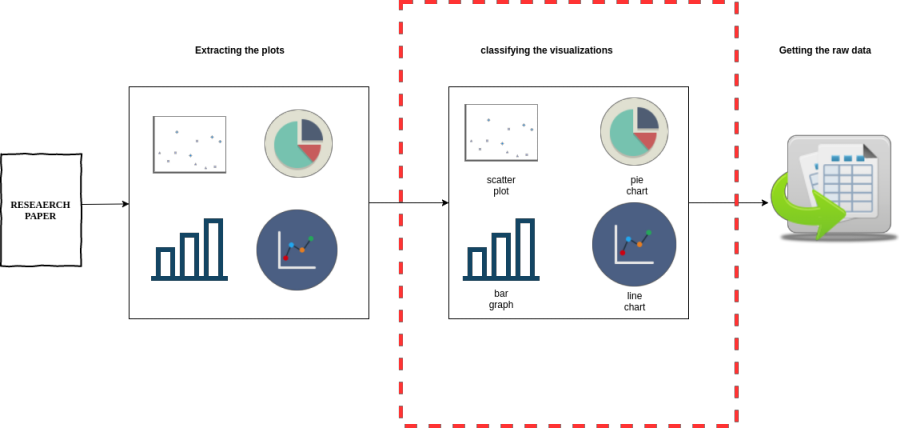
\includegraphics [scale=1.5] {vision}

\chapter{LITERATURE REVIEW}
Our work is inspired by Architecture proposal for data extraction of chart images using Convolutional Neural Network(2017), in this work a simple 
LeNet-based CNN model trained with four classes. The model was implemented using Tensorflow, and the model architecture was made of 3 convolutional layers, followed by a fully connected layer. The training process is based on the dataset divided into mini-batches, random samples of fixed sizes(100) are selected and used as input for the CNN, as different batches are used as the input the model keeps learning to generalize the classes of the dataset and therefore becomes more robust.Each image is converted to JPG and resized to 224x224x3 (using crop or pad), that is, 224 pixels of height, 224 of width and 3 layers of output (one for each RGB color channel). Additionally, the process was executed in 1000 epochs and the learning rate was set to 0.003. The accuracy of the final model was 70\%.

\section{Dataset}

\subsection{Dataset for Matlab}
The dummy data for creating the plots in Matlab were downloaded from Project Datasets \cite{wikiped} a site where datasets are provided in CSV formats for reasons of teaching people how to load datasets.
The datasets are multidimensional and complied from different fields. On the average the datasets used contain about 500 instance and 5 different columns. The biggest dataset is called Speed dating data with over 8,000 observations of matches and non-matches, with answers to survey questions about how people rate themselves and how they rate others on several dimensions. The smallest dataset
used is the Happiness dataset, it contains information about European quality of life survey with questions related to income, life satisfaction or perceived quality of society.

\subsection{Dataset for R}
For the plots in R, 13 random dummy csv files where download from an archive of datasets distributed with R \cite{Franklin1999} called Rdatasets. Rdatasets is a collection of 1147 datasets that were originally distributed alongside the statistical software environment R and some of its add-on packages, the main aim is to make these data more broadly accessible for teaching and statistical software development. On the average their are 80 instances and 5 columns. The biggest CSV file is the Australian athletes data set, these data were collected in a study of how data on various characteristics of the bloood varied with sport body size and sex of the athlete. It contains attributes like sex,height,weight and sports. The smallest dataset is the Canadian Women's Labour-Force Participation saved as the Bfox.csv file. The Bfox data frame has 30 rows and 7 columns, and contains Time-series data on Canadian women's labor-force participation, 1946–1975. It contains information like average wages of women, percent of adult women in the workforce etc.


\subsection{Dataset for PYTHON}
The dummy data used for creating the plots in Python were 15 randomly seleted csv files also from  Rdatasets \cite{Franklin1999}. The biggest dataset among the 15 is the Monoclonal gammapothy data, contains natural history of 1341 sequential patients with monoclonal gammapothy of undetermined significance (MGUS). The CSV is with 1384 observations with 10 columns with attributes like age,sex,time of death and last contact in months. On the average each dataset contains about 200 instances and 7 columns of multi-dimensional data. The smallest dataset however contains only 33 instances with 11 columns and is called the Nuclear Power Station Construction Data.The data relate to the construction of 32 light water reactor (LWR) plants constructed in the U.S.A in the late 1960's and early 1970's. The data was collected with the aim of predicting the cost of construction of further LWR plants.

\subsection{Dataset for Java}
For the java plots I used the dataset made available by Plotly \cite{wid}.They are CSV datasets used in the Plotly API examples.14 random CSV files were downloaded, the biggest file 3d-line-plot has 1002 instances and 9 columns, and on the average each file contains about 100 instances and 9 columns. The smallest file however is made of 33 instances and 12 columns called the mtcars file. It contain information about a variety of different car models like the number of gears, speed etc. 

\begin{table}[h]
	\centering \def\arraystretch{1.5} \small
	\begin{tabular}{|p{5cm}|p{3cm}|p{3cm}|p{4cm}|}
		
		 \hline
		 \multicolumn{4}{|c|}{DUMMY DATA} \\
		 \hline
				
		PYTHON & MATLAB & R LANGUAGE & JAVA\\ \hline
		
		3d\_line\_sample\_data.csv \par LightFordwardFlapStall.csv  \par line\_3d\_dataset.csv \par
		longley.csv  \par loti.csv  \par lung.csv  \par nuclear.csv  \par timeseries.csv  \par
		USJudgeRatings	\par WVSCulturalMap.csv  \par wind\_rose.csv  \par volcano.csv  \par uspop2.csvm &
		
		Camera.csv \par Cars.csv \par CausesOfDeath-France.csv \par Cereal.csv \par film.csv \par happiness.csv \par TestData1.csv \par TestData2.csv  \par mpg.csv \par okcupid-compatibility-religion.csv  \par spectral.csv
		\par stockdata.csv \par subplots.csv  & 
		
		ais.csv \par Angell.csv  \par Baumann.csv \par Bfox.csv \par cane.csv \par carprice.csv \par Chirot.csv
		Davis.csv \par Ericksen.csv \par Florida.csv \par Highway1.csv \par Pottery.csv \par Prestige.csv 
		salinity.csv \par urine.csv & 
		
		3d-line-plot.csv \par 3d-scatter.csv \par 2011\_flight\_paths.csv \par 2011\_us\_exports.csv \par auto-mpg.csv \par candlestick\_dataset.csv \par finance-charts-apple.csv \par 
		globe\_contours.csv\par hobbs-pearson-trials.csv \par motor\_trend\_tests.csv \par 
		nz\_weather.csv \par volcano.csv \par iris.csv \par mtcars.csv	\\ \hline
		

	\end{tabular}
	
	\caption {Names of CSV files used in each language}	\label{Table:1}
\end{table}


\chapter{CREATING PLOTS}
Scripts in various languages were written to handle the plotting and labeling process automatically. All datasets for a particular plot(example scatter plot for python) are put into one folder. The scripts reads each CSV file column by column. The first column is considered as the x-axis and its header the x-label and the next column will be the y-axis and its header the y-label, The y-axis then becomes the x-axis for the next plot and this process continues till all columns are used, while doing this all non numeric columns are ignored. 
Next the libraries used in creating the plots in various languages. For reading the values, the scripts written are done in a way to automatically create the plots. The inspiration for creating a variety of plots to capture all type of plots used in scientific papers was gotten by inspecting the dataset of this \cite{junior2017architecture} and \cite{lee2018viziometrics}. The tables below describe how the plots where created in each language, the plotting libraries used, the variants of a particular plot come under the type column, the parameter column describes parameters that were changed and finally the number of plots created were also added in the last column.


\begin{table}[h]
	\centering \def\arraystretch{1.5} \small
	
	\begin{tabular}{|p{3cm}|p{3cm}|p{3cm}|p{3cm}|p{3cm}|}
		
		\hline
		\multicolumn{5}{|c|}{SCATTER PLOTS} \\
		\hline
		
	Language & Library & Parameters &  Types & Number of plots\\ \hline
		
	Python  & Matplotlib v2.1.2 \par Plotly v2.5.1 \par Seaborn
		
		 v0.8.1 & MarkerStyle \par ['o', '*', '.', '+','x'] & \multirow{4}{*}{Normal scatter} &
		 
		  100\\ \hline	   
		  
	MATlAB   & Default &  MarkerStyle \par ['o', '*', '.', '+','x','s'] &   &  644 \\ \hline
		
	R LANGUAGE   & Default,Plotly \par R Library \par ggplot2 &  MarkerStyle \par ['o', '*', '.', '+','x','s'] &  &  644\\ \hline	
	
	JAVA   & XChart 3.5.1, & setMarkerSize (16) \par LegendPosition &   &  644\\ \hline
		  
	\end{tabular}
	
	\caption {How Scatter plots were created}	\label{Table:1}
\end{table}



\begin{figure}
	\begin{subfigure}{.5\textwidth}
		\centering
		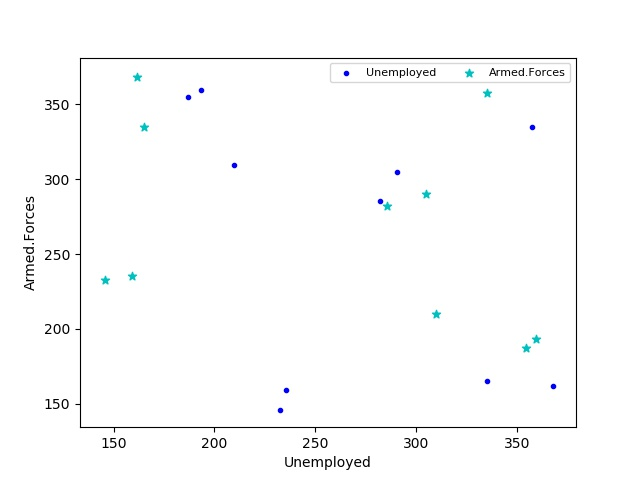
\includegraphics[width=.8\linewidth]{scatter1}
		\caption{created with Matplotlib}
		\label{fig:sfig1}
	\end{subfigure}%
	\begin{subfigure}{.5\textwidth}
		\centering
		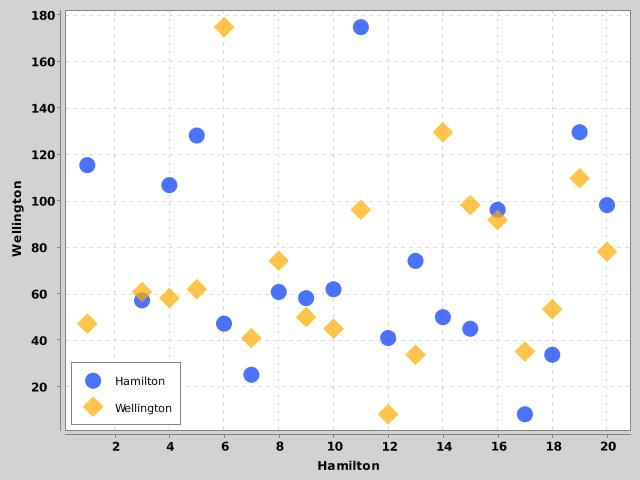
\includegraphics[width=.8\linewidth]{scatter2}
		\caption{created with Jfreechart library}
		\label{fig:sfig2}
	\end{subfigure}
	\caption{Example Scatter plots}
	\label{fig:fig}
\end{figure}




\begin{table}[h]
	\centering \def\arraystretch{1.5} \small
	
	\begin{tabular}{|p{3cm}|p{3cm}|p{3cm}|p{3cm}|p{3cm}|}
		
		\hline
		\multicolumn{5}{|c|}{BAR CHARTS} \\
		\hline
		
		Language & Library & Parameters &  Types & Number of plots\\ \hline
		
		Python  & Matplotlib v2.1.2 \par Plotly v2.5.1 \par Seaborn
		
		v0.8.1 &   &
		
		Horizontal and Vertical \par Stacked bar charts \par Grouped bar charts & 100\\ \hline
		
		MATlAB   & Default &  Width of bar &  &  644\\ \hline
		

		R LANGUAGE   & Default,Plotly \par R Library \par ggplot2 &  &   &  644\\ \hline
		
		JAVA   & XChart 3.5.1, & setMarkerSize (16) \par LegendPosition &   &  644\\ \hline
				
	\end{tabular}
	
	\caption {How Bar Charts were created}	\label{Table:1}
\end{table}



\begin{figure}
	\begin{subfigure}{.5\textwidth}
		\centering
		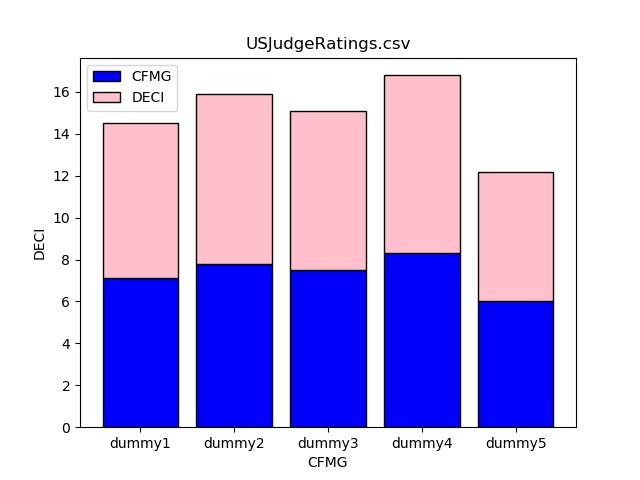
\includegraphics[width=.8\linewidth]{bar1}
		\caption{created in Matlab}
		\label{fig:sfig1}
	\end{subfigure}%
	\begin{subfigure}{.5\textwidth}
		\centering
		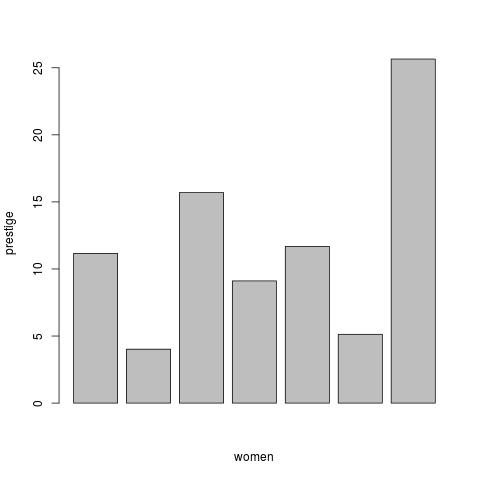
\includegraphics[width=.8\linewidth]{bar2}
		\caption{created in R}
		\label{fig:sfig2}
	\end{subfigure}
	\caption{Example Bar Charts}
	\label{fig:fig}
\end{figure}




\begin{table}[h]
	\centering \def\arraystretch{1.5} \small
	
	\begin{tabular}{|p{3cm}|p{3cm}|p{3cm}|p{3cm}|p{3cm}|}
		
		\hline
		\multicolumn{5}{|c|}{LINE CHARTS} \\
		\hline
		
		Language & Library & Parameters &  Types & Number of plots\\ \hline
		
		Python  & Matplotlib v2.1.2 \par Plotly v2.5.1 \par Seaborn
		
		v0.8.1 &   &
		
		Horizontal and Vertical \par Normal Line \par Lines with markers \par multiple lines  & 100\\ \hline
		
		MATlAB   & Default &  Width of bar &  &  644\\ \hline
		
		
		R LANGUAGE   & Default,Plotly \par R Library \par ggplot2 &  &  &  644\\ \hline
		
		JAVA   & XChart 3.5.1, &   &  &  644\\ \hline
		
	\end{tabular}
	
	\caption {How Line Charts were created}	\label{Table:1}
\end{table}


\begin{figure}
	\begin{subfigure}{.5\textwidth}
		\centering
		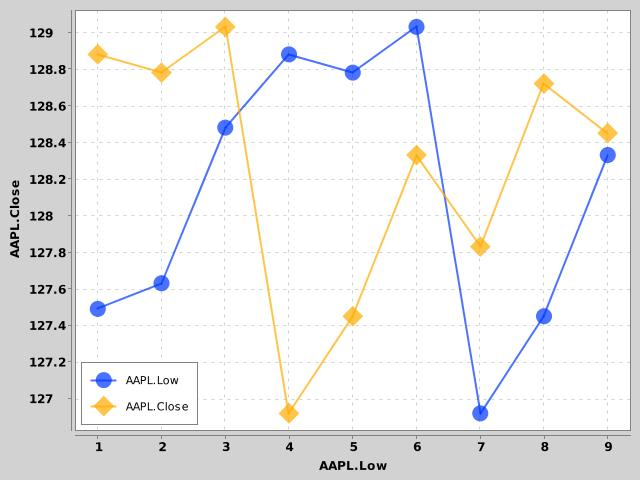
\includegraphics[width=.8\linewidth]{line1}
		\caption{created in Java}
		\label{fig:sfig1}
	\end{subfigure}%
	\begin{subfigure}{.5\textwidth}
		\centering
		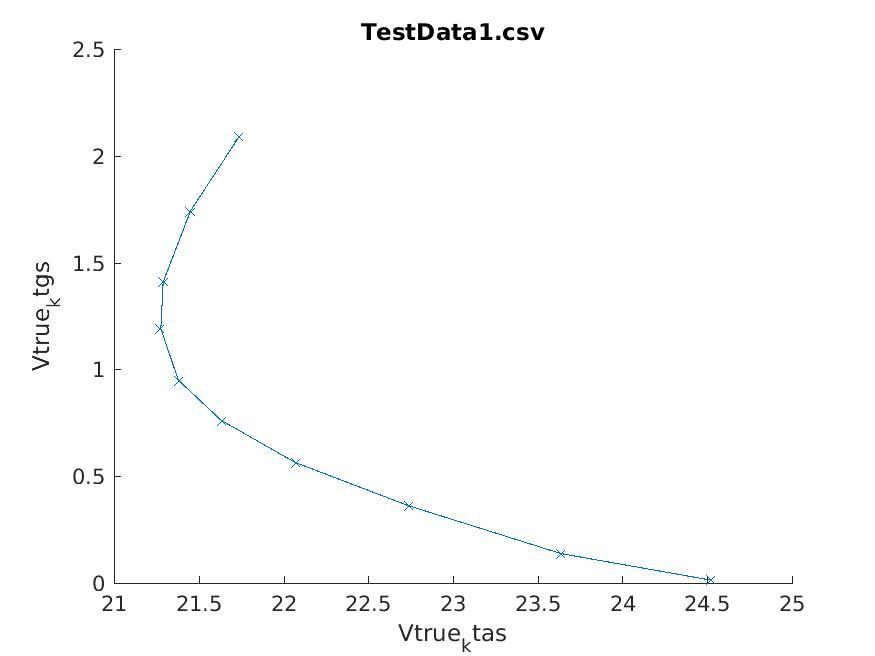
\includegraphics[width=.8\linewidth]{line2}
		\caption{created in Matlab}
		\label{fig:sfig2}
	\end{subfigure}
	\caption{Example Line Charts}
	\label{fig:fig}
\end{figure}



\begin{table}[h]
	\centering \def\arraystretch{1.5} \small
	
	\begin{tabular}{|p{3cm}|p{3cm}|p{3cm}|p{3cm}|p{3cm}|}
		
		\hline
		\multicolumn{5}{|c|}{BOX PLOTS} \\
		\hline
		
		Language & Library & Parameters &  Types & Number of plots\\ \hline
		
		Python  & Matplotlib v2.1.2 \par Plotly v2.5.1 \par Seaborn
		
		v0.8.1 &   &
		
		Horizontal and Vertical \par  Lines with markers \par multiple box plots  & 1000\\ \hline
		
		MATlAB   & Default &  &  &  644\\ \hline
		
		
		R LANGUAGE   & Default,Plotly \par R Library \par ggplot2 &  &  &  644\\ \hline
		
		JAVA   & XChart 3.5.1, &   &  &  644\\ \hline
		
	\end{tabular}
	
	\caption {How Box Plots were created}	\label{Table:1}
\end{table}



\begin{figure}
	\begin{subfigure}{.5\textwidth}
		\centering
		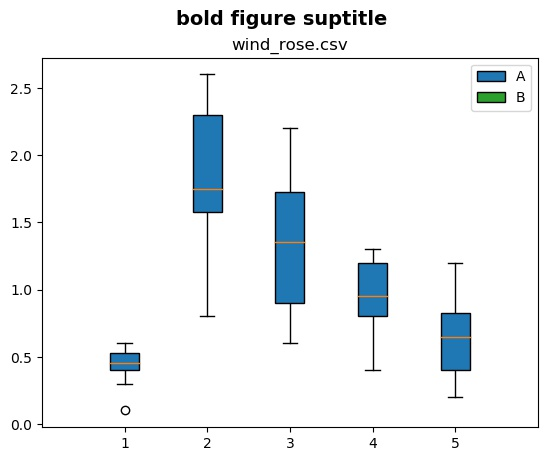
\includegraphics[width=.8\linewidth]{box1}
		\caption{created in python}
		\label{fig:sfig1}
	\end{subfigure}%
	\begin{subfigure}{.5\textwidth}
		\centering
		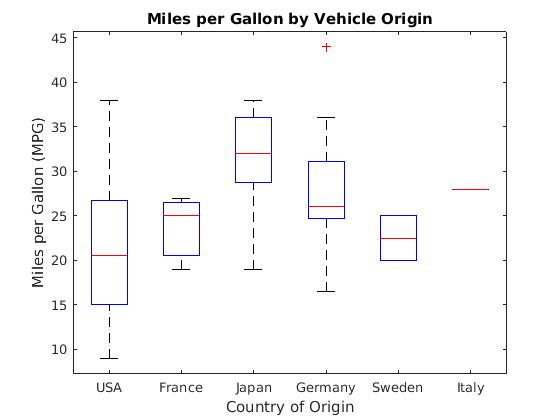
\includegraphics[width=.8\linewidth]{box2}
		\caption{created in Matlab}
		\label{fig:sfig2}
	\end{subfigure}
	\caption{Example Box Plots}
	\label{fig:fig}
\end{figure}



\section{Scatter plot}
For constructing the plots for the scatter plots I looked through a dataset from this paper[]. The dataset contained 555
scatter plots and looking through them I realized the markers used to plot where mainly zeros, triangles,squares,dots and x's.
So instead of just plotting all the markers randomly i plotted those mentioned above with a higher probability than the rest of the markers.
Also the scatter plots consisted of positive and negative correlation and just a few zero correlation. 
I also noticed that some markers were filled and other were not filled. So for creating my dataset I plotted with some markers being filled and other unfilled and this was done randomly. 

\section{Box Plots}

\bibliographystyle{unsrt}
\bibliography{sample}

\end{document}=====